\providecommand{\NA}{\textemdash}
\providecommand{\best}[1]{}
\renewcommand{\best}[1]{\begingroup\bfseries\boldmath #1\endgroup}
\providecommand{\second}[1]{}
\renewcommand{\second}[1]{\underline{#1}}
\begin{table*}[t!]
\centering
\footnotesize
\renewcommand{\arraystretch}{1.15}
\setlength{\tabcolsep}{5pt}
\begin{tabular}{@{}l*{6}{c}!{\hspace{5pt}\vrule width 0.45pt\hspace{5pt}}*{6}{c}@{}}
\BenchTopRule
\multirow{2}{*}{\textbf{Model}} & \multicolumn{6}{c!{\hspace{5pt}\vrule width 0.45pt\hspace{5pt}}}{\textbf{Overall Score} $\uparrow$} & \multicolumn{6}{c}{\textbf{Category Score@12h} $\uparrow$} \\
\BenchCMidRule{2-13}
 & @2h & @4h & @6h & @8h & @10h & \textbf{@12h} & Science & Code & Optimize & Knowledge & Math & Games \\
\BenchMidRule
Opus 4.8 & \best{39.0} & \best{45.7} & \best{48.1} & \best{49.8} & \best{50.9} & \best{51.3} & \best{48.5} & \best{67.4} & \best{36.5} & \best{47.0} & \best{55.0} & \best{39.3} \\
GPT-5.5 & \second{36.8} & \second{42.1} & \second{44.5} & \second{46.3} & \second{47.6} & \second{48.4} & \second{44.3} & \second{65.0} & \second{33.6} & \second{45.7} & \second{50.0} & \second{39.1} \\
GPT-5.4 & 29.7 & 34.0 & 36.5 & 38.0 & 38.9 & 39.3 & 33.5 & 54.1 & 27.9 & 38.8 & 40.8 & 29.0 \\
GLM-5.1 & 26.0 & 30.4 & 32.9 & 34.9 & 36.5 & 37.4 & 33.8 & 50.9 & 26.4 & 43.5 & 24.6 & 29.3 \\
DS-V4-Pro & 23.3 & 27.1 & 29.0 & 29.9 & 30.9 & 31.0 & 30.0 & 43.0 & 21.5 & 37.0 & 14.1 & 16.9 \\
\BenchBottomRule
\end{tabular}
\caption{Aggregate leaderboard. Overall scores are reported at each time budget, while category scores are reported at the 12-hour budget. Bold marks the best value in each score column and underlining marks the second-best value.}
\label{tab:aggregate_score_table}
\end{table*}


\section{Analysis of Environment Learning Dynamics}
\label{sec:analysis}

We study how frontier models perform and learn from environmental feedback over long horizons. We evaluate five frontier models: Claude Opus 4.8, GPT-5.5, GPT-5.4, GLM-5.1, and DeepSeek-V4-Pro (DS-V4-Pro). This section contains four analyses. Section~\ref{sec:frontier-comparison} compares frontier models at the aggregate, family, task, and submission levels. Section~\ref{sec:stateful-stateless-analysis} tests whether accumulated experience adds value beyond independent restarts. Section~\ref{sec:ralphloop} examines whether longer context still improves long-horizon interaction. Section~\ref{sec:case-study} traces a single scientific task to show how an agent's improvements unfold.
Appendix~\ref{sec:appendix-ablation-setting} reports additional harness-level continuation ablations for /goal mode and the Ralph loop.


\subsection{Comparison across Frontier Models}
\label{sec:frontier-comparison}

\underline{\textit{Setup.}} We follow Section~\ref{sec:environment-learning-data} and analyze 12-hour trajectories from two angles: \textbf{(1)} aggregate, family, and task performance, and \textbf{(2)} submission efficiency, i.e., how often submissions improve the current best result.

\begin{wrapfigure}{r}{0.48\textwidth}
\vspace{-0.8em}
\centering
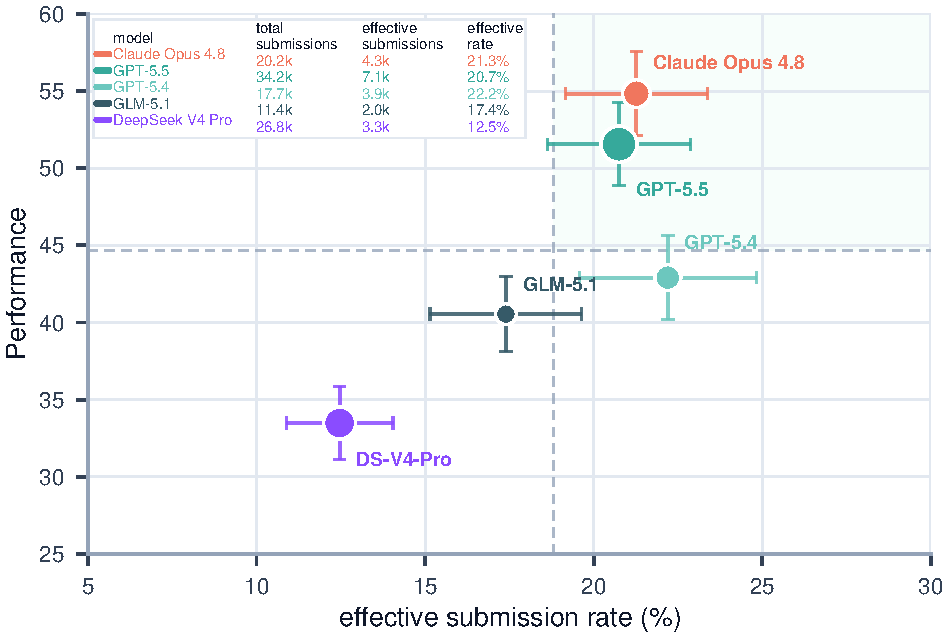
\includegraphics[width=\linewidth]{figures/analysis/conversion_performance_bubble.pdf}
\caption{12-hour effective-submission rate versus final performance. Marker area shows total submissions; error bars show task-level standard errors, and shading marks above-average rate and performance.}
\label{fig:effective-submission-performance}
\vspace{-1.0em}
\end{wrapfigure}

\underline{\textit{Performance Comparison.}} Table~\ref{tab:aggregate_score_table} gives the aggregate leaderboard over the 2 to 12 hour budget and reports family-level means at 12 hours. Claude Opus 4.8 leads throughout the time budget and reaches 51.3 at 12 hours, followed by GPT-5.5 at 48.4. GPT-5.4 and GLM-5.1 form the next tier at 39.3 and 37.4, while DS-V4-Pro obtains 31.0. Family-level results are broadly consistent with the aggregate ranking: Claude Opus 4.8 leads each family mean, with GPT-5.5 especially close in Games and second overall. Detailed per-task performance is reported in Appendix~\ref{sec:appendix-category-scores}, with~$\ast$ marking cells based on fewer than three valid runs.

\underline{\textit{Submission efficiency.}} We count each agent submission and mark it as effective when it sets a new best-so-far score. Figure~\ref{fig:effective-submission-performance} compares each model's 12-hour effective-submission rate with its final performance. Models that make more effective submissions usually perform better, but more submissions do not automatically lead to a better final result. \textbf{Claude Opus 4.8 achieves the best final performance despite submitting less often than GPT-5.5}, and GPT-5.4 has the highest effective-submission rate but still trails the top two models. Progress therefore depends not only on how often an agent improves its score, but also on whether those improvements are large, reliable, and reusable. Stronger agents use feedback more deliberately: they build a submit-ready baseline, preserve the current best solution, make focused changes, and use feedback to keep gains or roll back failures. Weaker agents more often over-trust local proxies, bundle unrelated edits, or continue broad exploration after feedback has ruled out a direction, reducing sample efficiency.

\subsection{Agents Do Learn from Experience beyond Repeated Sampling}
\label{sec:stateful-stateless-analysis}

\underline{\textit{Motivation.}} A rising best-so-far curve does not by itself prove that an agent is learning. Running longer also gives more chances to stumble on a good solution: with enough independent tries, the best of them climbs by luck alone. We therefore test whether the agent's accumulated experience adds value beyond such repeated sampling under the same total time budget.

\underline{\textit{Setup.}} We give Opus 4.8 the same 12-hour budget on each of 17 tasks and compare two ways of spending it, \textit{with} versus \textit{without} accumulated experience. \textbf{With experience}: the agent runs once and continuously, keeping its workspace, artifacts, and feedback history throughout, so experience builds up across the whole run. \textbf{Without experience}: the same budget is split into \(n=6\) independent attempts of \(\tau=2\) hours, with all state discarded between attempts and only the best result kept, so each attempt starts from scratch and any gain can come only from repeated sampling. Comparing the two at elapsed time \(t=k\tau\) contrasts one continuous run after \(t\) hours against the best of \(k\) independent attempts using the same total time. Appendix~\ref{sec:experience-gain-estimation} details how each curve is estimated.

\underline{\textit{Result.}} Figure~\ref{fig:stateful-stateless-gain} shows a clear gain from experience: the with-experience curve stays above the without-experience baseline under the same time budget. At 12 hours it reaches 43.0 versus 36.1, a gain of \(+6.9\). The improvement is therefore not explained by repeated sampling alone: accumulating and reusing task experience drives progress beyond what independent restarts achieve.

\begin{figure}[!tbp]
\centering
\begin{subfigure}[t]{0.49\linewidth}
\centering
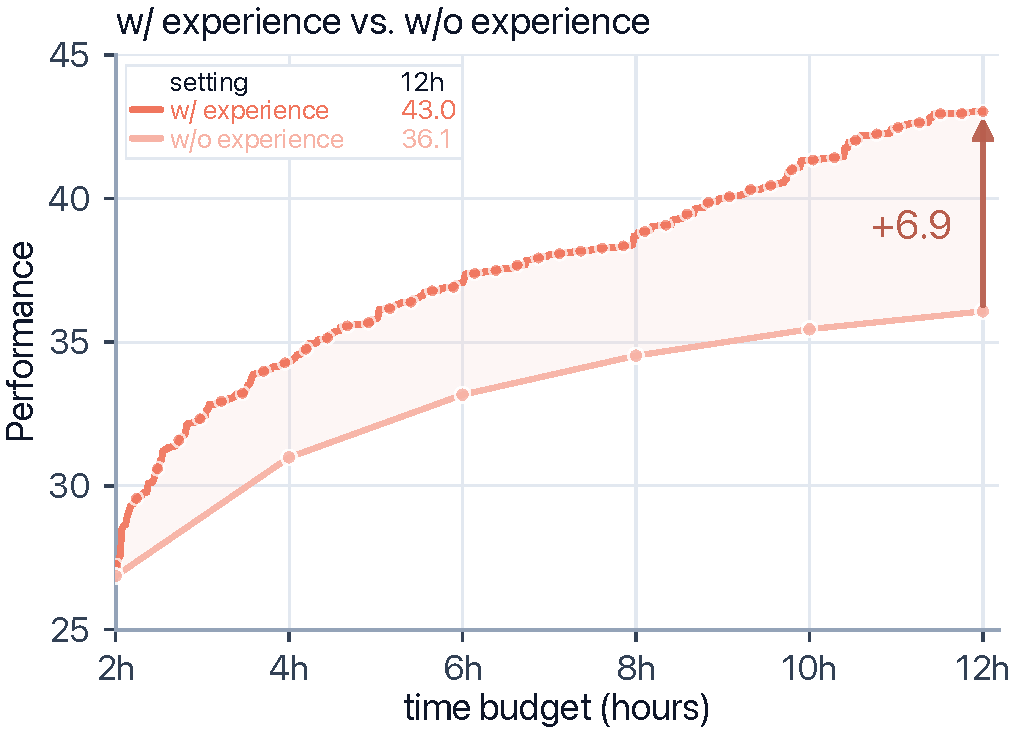
\includegraphics[width=\linewidth]{figures/ablation/stateful_stateless_gain_ablation.pdf}
\phantomcaption
\label{fig:stateful-stateless-gain}
\end{subfigure}
\hfill
\begin{subfigure}[t]{0.49\linewidth}
\centering
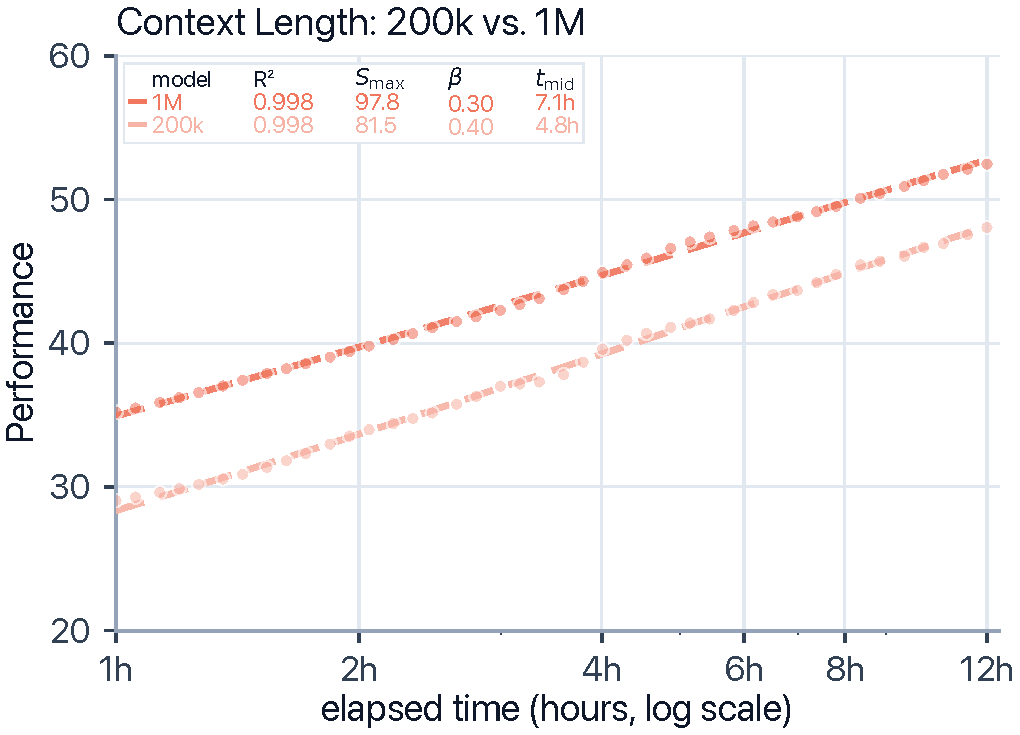
\includegraphics[width=\linewidth]{figures/ablation/opus_context_scaling_ablation.pdf}
\phantomcaption
\label{fig:opus-context-scaling-ablation}
\end{subfigure}
\vspace{-1.1em}
{\footnotesize
\centering
\setlength{\tabcolsep}{3pt}
\renewcommand{\arraystretch}{1.05}
\begingroup
\arrayrulecolor{black}
\begin{minipage}[t]{0.49\linewidth}
\centering
\begin{tabular}{@{}>{\raggedright\arraybackslash}p{0.46\linewidth}*{3}{>{\raggedright\arraybackslash}p{0.14\linewidth}}@{}}
\BenchTopRule
{} & 2h & 6h & 12h \\
\BenchMidRule
w/o experience & 26.9 & 33.2 & 36.1 \\
w/ experience & 27.2\textsubscript{+0.4} & 37.1\textsubscript{+3.9} & 43.0\textsubscript{+6.9} \\
\BenchBottomRule
\end{tabular}
\end{minipage}%
\hfill
\begin{minipage}[t]{0.49\linewidth}
\centering
\makebox[\linewidth][c]{%
\hspace*{0.06\linewidth}%
\begin{tabular}{@{}>{\raggedright\arraybackslash}p{0.42\linewidth}*{3}{>{\raggedright\arraybackslash}p{0.15\linewidth}}@{}}
\BenchTopRule
{} & 2h & 6h & 12h \\
\BenchMidRule
Opus 4.8 200k & 33.8 & 42.6 & 48.0 \\
Opus 4.8 1M & 39.6\textsubscript{+5.8} & 48.0\textsubscript{+5.5} & 52.5\textsubscript{+4.4} \\
\BenchBottomRule
\end{tabular}
}
\end{minipage}
\arrayrulecolor{black}
\endgroup
}
\vspace{0.55em}
\caption{\textbf{Left:} Gain from accumulated experience for Opus 4.8: the w/ experience run minus the w/o experience baseline (independent restarts) under the same total time budget. \textbf{Right:} Context-length ablation: 200k vs. 1M on Opus 4.8. Each curve shows the average performance over time; dashed lines are log-sigmoid fits.}
\label{fig:ablation-panels}
\vspace{-0.8em}
\end{figure}

\subsection{How Much Does a Longer Context Improve Performance}
\label{sec:context-length-analysis}
\label{sec:ralphloop}

\underline{\textit{Motivation.}} Section~\ref{sec:stateful-stateless-analysis} shows that accumulated experience can improve performance. A remaining question is how this experience should be retained during a long run. Using long context is a natural way to do so. However, frontier-agent harnesses can also maintain state outside the model context through workspace files, compaction, progress notes, and memory-like artifacts. It is therefore unclear whether extending the context window still provides additional benefits once these external state channels are available, and if so, by how much.

\underline{\textit{Setup.}} We compare 200k-context Opus 4.8 with 1M-context Opus 4.8 on the 42-task subset under the same long-horizon evaluation protocol.

\underline{\textit{Result.}} A longer context yields a consistent multi-point gain throughout the 12-hour window (Figure~\ref{fig:opus-context-scaling-ablation}). The 1M-context Opus 4.8 stays above the 200k variant at every checkpoint, and the two trajectories run roughly parallel: the gap is $+5.8$ at 2h and only edges down to $+4.4$ by 12h, with both curves well described by the same log-sigmoid form. Thus, even with identical external workspace and harness state, a longer context window gives a stable advantage over the horizon, with at most a slight tendency to narrow.

\subsection{Case Study}
\label{sec:case-study}

\underline{\textit{Setup.}} We examine the gravitational-wave reconstruction task. Based on the first GW150914 detection paper~\cite{abbott2016observation}, the agent must recreate the published signal analysis from LIGO strain data. The target has three output groups: H1/L1 waveforms, H1/L1 spectrograms, and velocity/separation curves for the source dynamics. The judge weights the five component scores at 0.15 for each waveform, 0.20 for each spectrogram, and 0.30 for velocity/separation. We run a Codex agent with periodic auto-evaluation, auto-resume, no Internet access, a 30-minute evaluation interval, and a 120-second submission cooldown. The agent made 224 explicit submissions, the harness added 23 auto-evaluations, and the run timed out at the 12-hour budget.

\begin{figure}[!t]
\centering
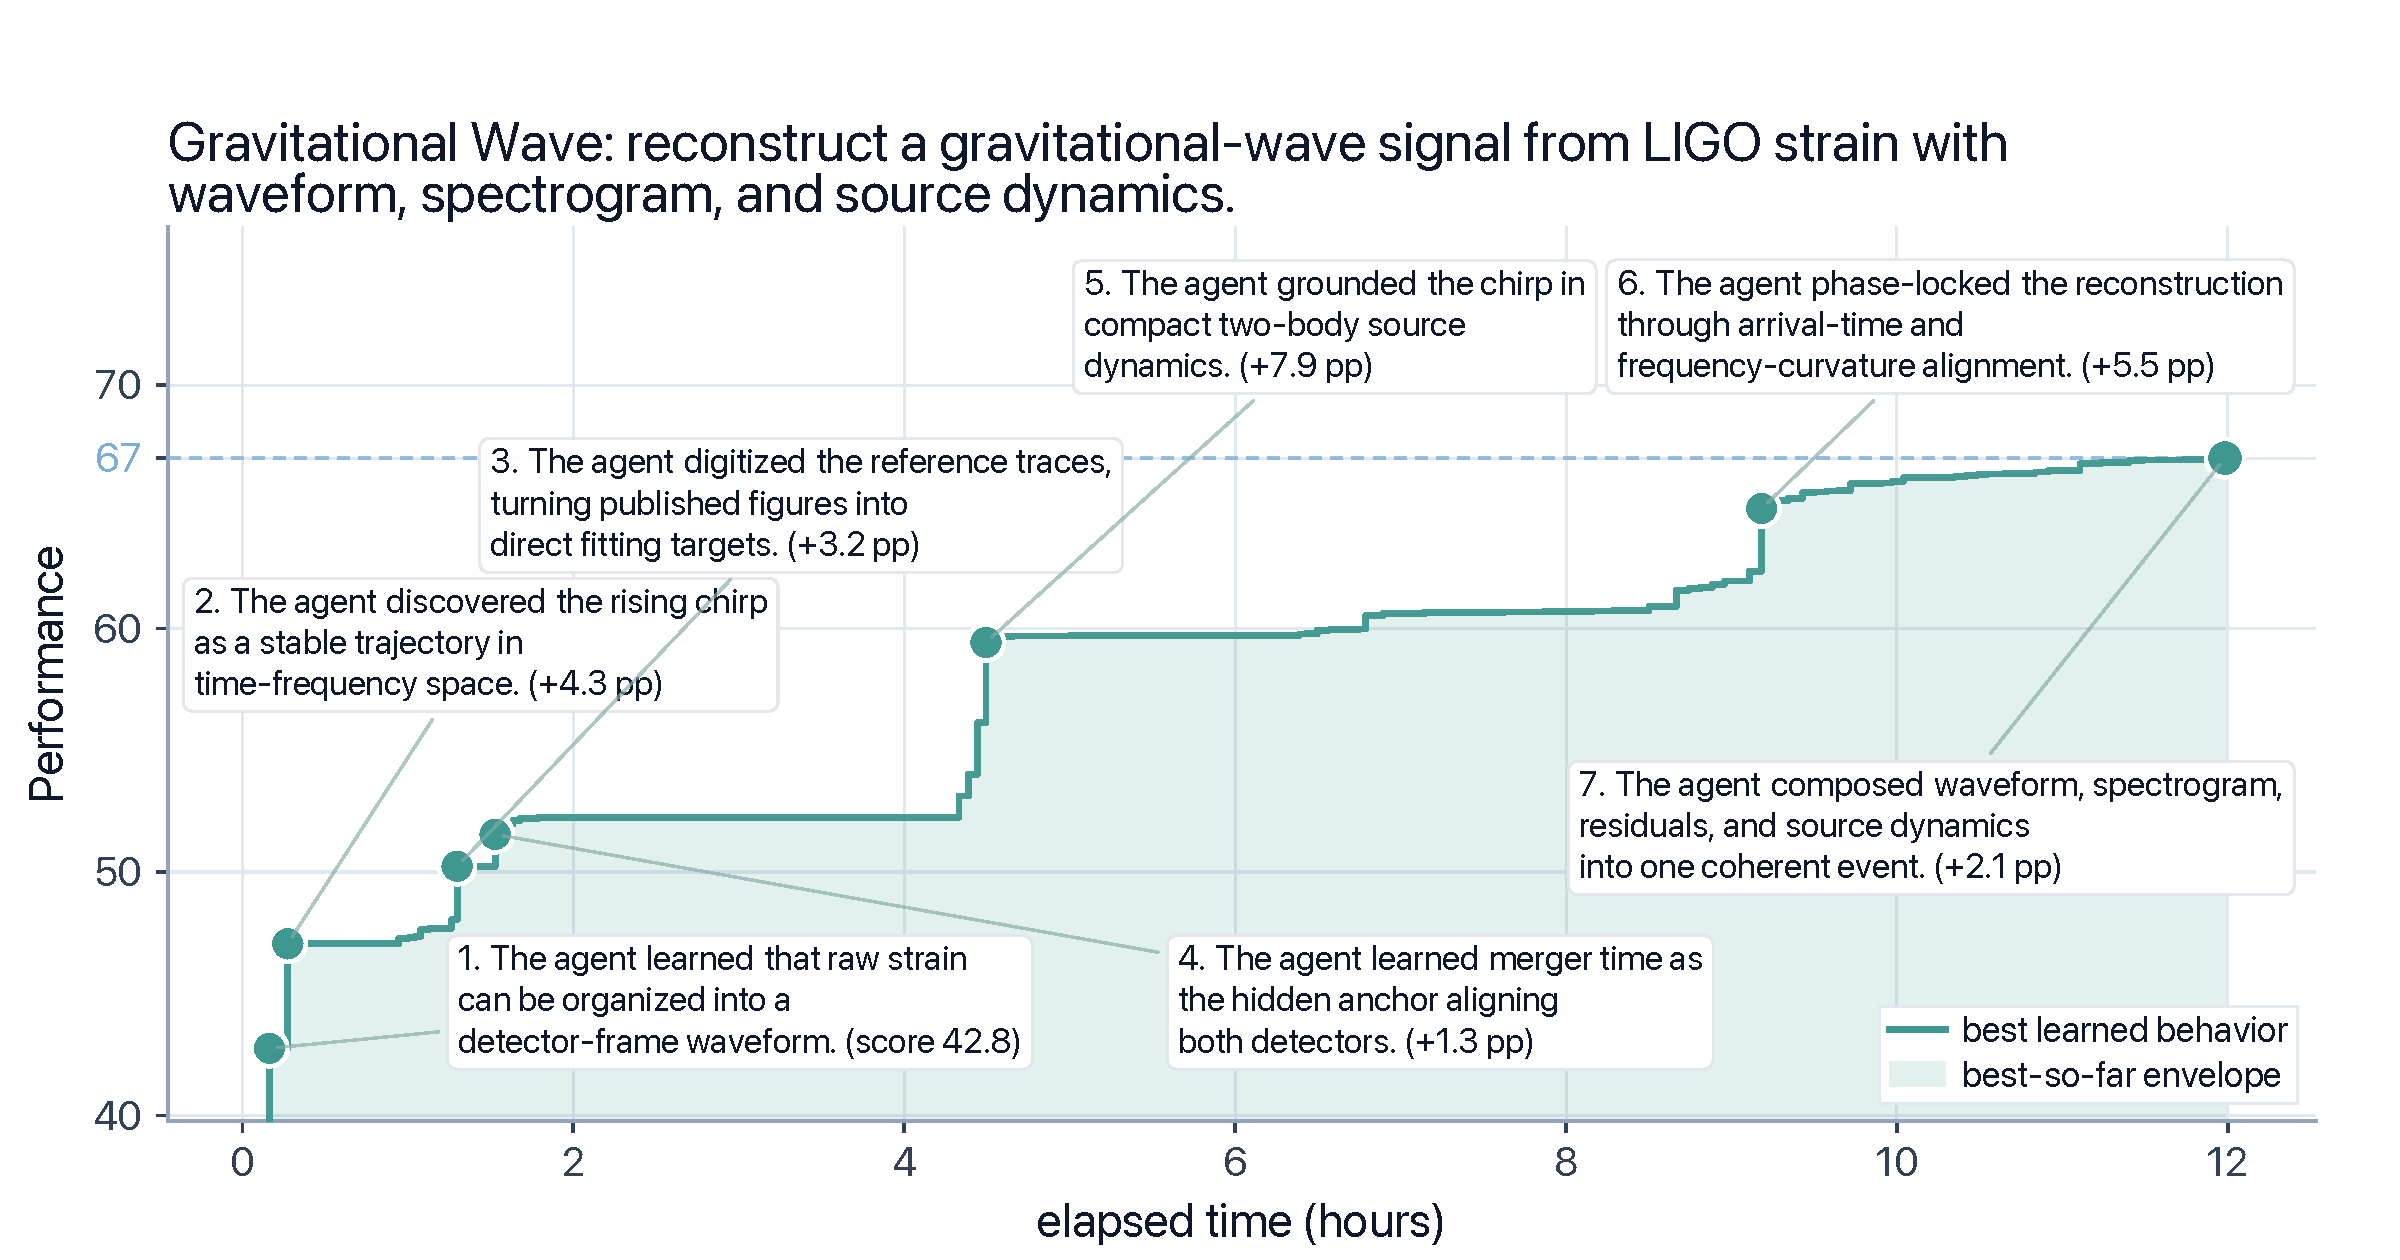
\includegraphics[width=\linewidth]{figures/case_study/gravitational_wave_case_study.pdf}
\caption{Gravitational-wave reconstruction task case study. The trajectory shows how a GPT-5.5 agent improves over a 12-hour run, with numbered milestones marking representative best-so-far updates.}
\label{fig:gw-case-study}
\end{figure}

\textbf{The trajectory reveals a sparse but structured diagnose-edit-evaluate loop.} The loop is sparse because most submissions are exploratory probes: only 27 of 224 agent submissions improve the best-so-far score by at least 0.1 percentage points. It is structured because feedback repeatedly changes what the agent searches for. The agent first makes the task measurable, then breaks unresolved errors into smaller searches, then identifies a main bottleneck and keeps searching around it, and finally keeps a working solution while repairing the remaining errors. These patterns show how many failed trials can still produce a small number of cumulative improvements.

\begin{itemize}
\item \textbf{The agent first makes the problem measurable before making it better.} The first valid submission turns an underspecified analysis task into a scoreable pipeline, but feedback exposes weak source dynamics. The agent then spends the first 11 submissions stabilizing the pipeline and replacing a noisy frequency estimate, producing three meaningful updates and a +4.5 pp gain.
\item \textbf{When direct repair stalls, the agent decomposes the failure into searchable subproblems.} Instead of treating waveform mismatch as one opaque error, the agent separates reference anchoring, time-frequency localization, and detector alignment. Across 40 signal-search submissions, this decomposition yields seven meaningful updates and lifts the best score to 52.3.
\item \textbf{Identifying a main bottleneck lets the agent keep searching productively.} After broad signal-processing edits plateau, component feedback identifies velocity/separation as the dominant gap. The agent keeps searching within source-mass calibration rather than rewriting the whole pipeline; in the 4--5h window, 17 submissions and five useful updates raise source dynamics from 64.2 to 89.0, creating the largest jump in the run.
\item \textbf{After finding a stable solution, the agent keeps the core and repairs only the remaining errors.} In the final hours, most residual edits fail to transfer. Instead of restarting the pipeline, the agent keeps the source model fixed and tests targeted residual corrections, phase alignment, and narrow-band corrections. These useful updates raise the H1 waveform component score from roughly 47 to 95, while the aggregate best score reaches 67.0.
\end{itemize}

\textbf{The run improves through uneven jumps rather than a smooth climb.} Across 247 scored evaluations, the best score rises from 42.8 to 67.0 on the 0--100 scale. Figure~\ref{fig:gw-case-study} shows seven representative milestones. These jumps correspond to the behavior patterns above: the agent first makes the task scoreable, then localizes the signal, improves source dynamics, and finally repairs the remaining H1 waveform errors. Detailed milestone phases and final subscore composition are reported in Appendix~\ref{sec:appendix-gw-case-study-details}.
